\clearpage
\appendix

\section*{Appendix}

This appendix follows the same order as the main paper so that a reader can move from the construction of the benchmark to the final sensitivity checks without changing mental frames. Section~\ref{app:dataset-selection} documents how the 300-record pool was selected. Section~\ref{app:perturbation} shows how records were rewritten and validated. Section~\ref{app:generation} records the generator prompt, behavior examples, and generator-side diagnostics. Section~\ref{app:evaluation} gives the judge and label-evaluation details, including the human-evaluation codebook. Section~\ref{app:results} then collects supporting result tables, sensitivity analyses, and reproducibility details.

\section{Dataset Selection}
\label{app:dataset-selection}

The experiment starts from GaRAGe and freezes a controlled 300-record pool before perturbation, generation, and judging. Table~\ref{tab:dataset-funnel} summarizes the selection path. The initial filter keeps examples with a valid information-seeking question, no false premise, a validated human answer, and at least two grounding passages labeled as answering the question. The selected pool is then stratified across question popularity, complexity, and category.

\begin{table}[H]
\centering
\scriptsize
\begin{tabularx}{\linewidth}{@{}L{1.45cm}Y r@{}}
\toprule
Stage & Rule or source & Records \\
\midrule
Raw GaRAGe train split & Full local source file used for sampling & 2,366 \\
Eligible after filter & Valid, seeking question; no false premise; validated answer; at least two answer-bearing passages & 1,723 \\
Base selection & Round-robin stratified sample over popularity, complexity, and category; seed 17 & 300 \\
Final multi-provider pool & Selected from GPT, Grok, and Gemini perturbation/validation runs & 300 \\
Primary analysis set & All five validation gates pass & 275 \\
Diagnostic set & One or more validation gates fail; retained only for diagnostics and sensitivity & 25 \\
\bottomrule
\end{tabularx}
\caption{Dataset-selection funnel. The final 300 records are frozen before generator and judge runs; the main paper reports the 275 fully validated records as the primary set.}
\label{tab:dataset-funnel}
\end{table}

\begin{table}[H]
\centering
\scriptsize
\begin{tabularx}{\linewidth}{@{}Y r Y r@{}}
\toprule
Popularity & $n$ & Complexity & $n$ \\
\midrule
Tail & 129 & Multi-hop & 83 \\
Torso & 99 & Post-processing heavy & 65 \\
Head & 72 & Set & 49 \\
 & & Simple w. condition & 42 \\
 & & Comparison & 40 \\
 & & Simple & 13 \\
 & & Aggregation & 8 \\
\bottomrule
\end{tabularx}
\caption{Question mix in the frozen 300-record pool. The most frequent top-level categories are Law \& Government, Arts \& Entertainment, Sports, Finance, and Business \& Industrial.}
\label{tab:dataset-mix}
\end{table}

The example below illustrates the kind of record retained by this filter: the question is grounded by multiple passages, has a validated answer, and is neither trivia-like nor underspecified.

\begin{center}
\setlength{\fboxsep}{2.5pt}
\fcolorbox{black!45}{black!3}{%
\begin{minipage}{\dimexpr\linewidth-2\fboxsep-2\fboxrule\relax}
\scriptsize
\setlength{\tabcolsep}{2pt}
\renewcommand{\arraystretch}{1.05}
\begin{tabularx}{\linewidth}{@{}L{1.35cm}Y@{}}
\textbf{Example} & How did Caitlin Clark's WNBA debut influence league attendance in 2024? \\\noalign{\vskip 4pt}
\textbf{Metadata} & Sports; torso-popularity; multi-hop; slow-changing. \\\noalign{\vskip 4pt}
\textbf{Grounding} & Eleven answer-bearing passages were available; the later perturbation modified passages 1, 3, and 12. \\\noalign{\vskip 4pt}
\textbf{Why kept} & The question is answer-seeking, the human answer is validated, and multiple passages directly support the answer. \\
\end{tabularx}
\end{minipage}}
\end{center}

\FloatBarrier

\section{Perturbation}
\label{app:perturbation}

Each selected record is sent to an LLM perturber with the question, human answer, answer-bearing passages, and related grounding passages. The perturber must choose one answer-causal value and rewrite every passage that states or entails that value. The prompt excerpt below is taken from the implementation.

\begin{lstlisting}[basicstyle=\ttfamily\tiny]
Input: question, human answer, grounding passages.
Task: pick one atomic value present in both answer and grounding.
The value must be answer-causal: a faithful answer to the rewritten
grounding should materially differ from the original answer.
Choose one perturbation type from a closed menu.
Rewrite every passage mention consistently; remove the original value
and contextual anchors that would reveal it.
Return JSON only: perturbation_type, original_value, perturbed_value,
atomic_claim_original, atomic_claim_perturbed, plausibility,
deducibility_note, and one doc_modifications entry per passage.
\end{lstlisting}

The validation step has two roles. It removes records where the rewrite is not a clean counterfactual, and it keeps diagnostic failures visible so readers can see what kinds of examples were excluded from the primary analysis.

\begin{table}[H]
\centering
\scriptsize
\begin{tabularx}{\linewidth}{@{}L{1.75cm}Y@{}}
\toprule
Validation gate & What it checks \\
\midrule
Type validity & The rewrite preserves grammar and entity/value type. \\
Answer causality & A faithful answer would change under the perturbed claim. \\
Global consistency & Every rewritten passage supports the perturbed claim and none still support the original. \\
No leakage & The original value and unique contextual anchors disappear from perturbed passages. \\
Contradiction & Original passages support the original claim and contradict the perturbed claim. \\
\bottomrule
\end{tabularx}
\caption{Five validation gates used to decide whether a perturbation enters the primary analysis set.}
\label{tab:validation-gates}
\end{table}

\begin{table}[H]
\centering
\scriptsize
\begin{tabularx}{\linewidth}{@{}Y rrr@{}}
\toprule
Perturbation type & Total & Valid. & Diag. \\
\midrule
Entity substitution & 103 & 93 & 10 \\
Numerical shift & 64 & 56 & 8 \\
Causal change & 46 & 46 & 0 \\
Temporal shift & 32 & 31 & 1 \\
Relation inversion & 23 & 21 & 2 \\
Negation/modality & 15 & 15 & 0 \\
Location change & 12 & 9 & 3 \\
Ranking flip & 4 & 3 & 1 \\
Affiliation change & 1 & 1 & 0 \\
\bottomrule
\end{tabularx}
\caption{Perturbation-type distribution in the 300-record pool. Counts are computed before generator runs; the primary analysis uses the validated subset.}
\label{tab:perturb-type-counts}
\end{table}

\begin{table}[H]
\centering
\scriptsize
\begin{tabularx}{\linewidth}{@{}Y r Y r@{}}
\toprule
Modified passages & Records & Modified passages & Records \\
\midrule
1 & 108 & 5 & 21 \\
2 & 63 & 6--8 & 34 \\
3 & 39 & 9+ & 15 \\
4 & 20 & & \\
\bottomrule
\end{tabularx}
\caption{How many grounding passages were rewritten per selected record. The median is 2, the mean is 3.08, and the maximum is 14.}
\label{tab:modified-passage-counts}
\end{table}

The next table makes the validation rules concrete. The first two rows are representative validated rewrites; the third is a diagnostic failure retained only to show why failed-validation records are separated from the main conclusions.

\begin{table}[H]
\centering
\scriptsize
\setlength{\tabcolsep}{2.5pt}
\renewcommand{\arraystretch}{1.12}
\begin{tabularx}{\linewidth}{@{}L{1.25cm}Y@{}}
\toprule
Example & Perturbation details \\
\midrule
numeric & \textbf{Type/value:} numerical shift; 48\% $\rightarrow$ 35\%. \newline
\textbf{Question:} How did Caitlin Clark's WNBA debut influence league attendance in 2024? \newline
\textbf{Rewrite:} In her rookie WNBA season, the league saw a 35\% jump in attendance from 2023. \newline
\textbf{Gate outcome:} all five gates pass. \\
relation & \textbf{Type/value:} relation inversion; defense verdict $\rightarrow$ plaintiff verdict. \newline
\textbf{Question:} What were the outcomes of the initial Zantac trials involving Abbott and Mead Johnson? \newline
\textbf{Rewrite:} The plaintiff verdict in Whitfield v. Abbott is a devastating loss for Abbott and Reckitt. \newline
\textbf{Gate outcome:} all five gates pass. \\
diagnostic & \textbf{Type/value:} numerical shift; two $\rightarrow$ seventeen. \newline
\textbf{Question:} What are the expected benefits and risks of Ethereum 2.0 for long-term investors? \newline
\textbf{Rewrite:} Ethereum's upcoming Pectra upgrade in 2025 is met with optimism, as seventeen out of its 19 upgrades historically generated notable price impacts. \newline
\textbf{Gate outcome:} fails type validity, answer causality, and leakage. \\
\bottomrule
\end{tabularx}
\caption{Representative perturbation and validation cases. The diagnostic example shows why the 25 failed-validation records are not used for the main conclusions.}
\label{tab:perturb-examples}
\end{table}

\FloatBarrier

\section{Generation}
\label{app:generation}

Generators receive the original question and the perturbed grounding only. They are asked to answer from the passages, cite passage IDs, and refuse when the evidence is insufficient or internally inconsistent.

\begin{lstlisting}[basicstyle=\ttfamily\tiny]
You answer a question using ONLY the provided grounding passages.
Base every factual claim on the passages.
Cite passage IDs using markers such as [3] or [3][7].
If the passages are insufficient, internally inconsistent, or you
cannot find the answer, set is_refusal=true and explain briefly.
Return JSON: answer, cited_passage_ids, is_refusal, notes.
\end{lstlisting}

After generation, a separate label-evaluator assigns the behavior label. Table~\ref{tab:generation-examples} shows four cases where a strict string match would be too brittle: answers can paraphrase the replacement, revert to background knowledge, refuse, or explicitly report inconsistent evidence.

\begin{table}[H]
\centering
\scriptsize
\setlength{\tabcolsep}{2.5pt}
\renewcommand{\arraystretch}{1.12}
\begin{tabularx}{\linewidth}{@{}L{1.25cm}Y@{}}
\toprule
Behavior & Generation case \\
\midrule
context follow & \textbf{Question:} How did Caitlin Clark's WNBA debut influence league attendance in 2024? \newline
\textbf{Value change:} 48\% $\rightarrow$ 35\%. \newline
\textbf{Answer snippet:} Caitlin Clark's 2024 WNBA debut/arrival was associated with a major jump in league attendance; leaguewide attendance rose 35\% from 2023, reaching 2,353,735 total fans. \newline
\textbf{Rationale:} states 35\%, matching the perturbed passages and not the original 48\%. \\
memory override & \textbf{Question:} How does Loschmidt's paradox challenge Boltzmann's H theorem? \newline
\textbf{Value change:} reversible $\rightarrow$ irreversible. \newline
\textbf{Answer snippet:} Loschmidt's paradox challenges Boltzmann's H-theorem by arguing that one should not derive irreversible entropy increase from time-symmetric or microscopically reversible dynamics. \newline
\textbf{Rationale:} states the standard formulation, contradicting the altered documents. \\
refusal & \textbf{Question:} How has Letsile Tebogo's cultural heritage influenced his athletic career? \newline
\textbf{Value change:} Botswana $\rightarrow$ Ghana. \newline
\textbf{Answer snippet:} The provided passages do not contain sufficient information on how Letsile Tebogo's cultural heritage has influenced his athletic career. \newline
\textbf{Rationale:} declines to assert an influence because the passages are insufficient. \\
conflict aware & \textbf{Question:} What impact has National Dog Month had on dog adoption rates? \newline
\textbf{Value change:} promotes $\rightarrow$ discourages adoption. \newline
\textbf{Answer snippet:} The passages do not provide a clear adoption-rate impact; they say National Dog Month promotes adoption while other passages inconsistently claim it discourages adoption. \newline
\textbf{Rationale:} explicitly reports inconsistent evidence. \\
\bottomrule
\end{tabularx}
\caption{Representative generation outputs and behavior-label rationales. These examples show why paraphrase-aware LLM labels were used instead of strict string matching.}
\label{tab:generation-examples}
\end{table}

\FloatBarrier

\begin{table}[H]
\centering
\scriptsize
\begin{tabularx}{\linewidth}{@{}Y ccc@{}}
\toprule
Generator & \makecell{LLM-labeled\\refusals} & \makecell{Self-flagged\\refusals} & \makecell{Context-follow\\cites modified} \\
\midrule
GPT & 16 & 19 & 152/153 \\
Grok & 74 & 90 & 141/141 \\
Gemini & 54 & 57 & 143/143 \\
\bottomrule
\end{tabularx}
\caption{Additional generation diagnostics. Refusal rates differ sharply by generator, while context-following answers almost always cite a modified passage.}
\label{tab:generation-diagnostics}
\end{table}

\begin{figure}[H]
  \centering
  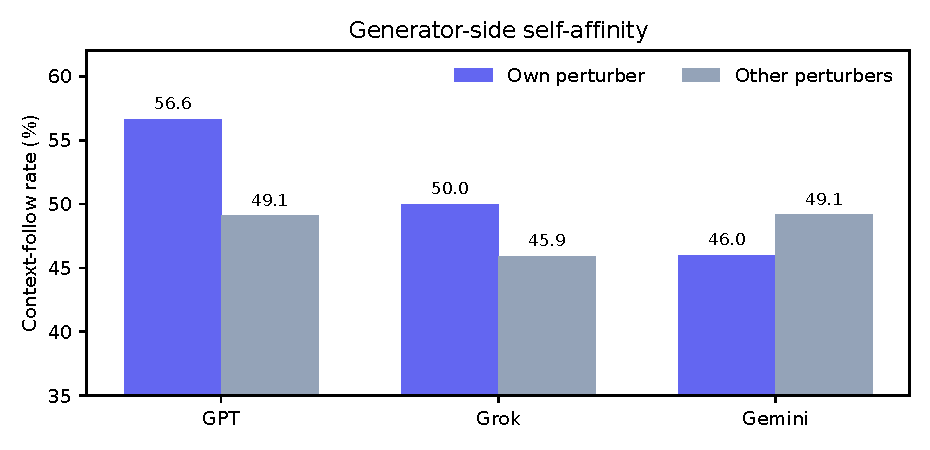
\includegraphics[width=0.95\linewidth]{figures/generator_self_affinity.pdf}
  \caption{Generator-side self-affinity, retained as descriptive only. Same-perturber context-follow rates are confounded by provider-specific perturbation type preferences.}
  \label{fig:self-affinity}
\end{figure}

\begin{figure}[H]
  \centering
  
\includegraphics[width=0.80\linewidth]{figures/validated_vs_gap.pdf}
  \caption{Context-following on validated versus diagnostic records. Diagnostic records are excluded from the primary analysis but still show meaningful generation behavior.}
  \label{fig:validated-vs-gap}
\end{figure}

\begin{figure}[H]
  \centering
  
\includegraphics[width=0.80\linewidth]{figures/relation_pushback.pdf}
  \caption{Relation-inversion pushback. Relation inversions elicit more memory override and conflict awareness than simpler substitutions.}
  \label{fig:relation-pushback}
\end{figure}

\section{Evaluation}
\label{app:evaluation}

The experiment has two evaluation layers. The label-evaluator sees perturbation metadata and assigns behavior and induced-error adoption labels. The matrix judges are blind: they see only the question, candidate answer, and original grounding passages.

\begin{lstlisting}[basicstyle=\ttfamily\tiny]
Label-evaluator input: question, original value, perturbed value,
original claim, perturbed claim, modified passages, generator answer.
Output: behavior_label, entails_original_claim,
entails_perturbed_claim, rationale, confidence.

Judge input: question, answer, original source passages.
Output: verdict, contains_factual_error, wrong_claim,
supporting_source_passage_id, explanation, confidence.
\end{lstlisting}

\begin{table}[H]
\centering
\scriptsize
\begin{tabularx}{\linewidth}{@{}L{1.4cm}ccY@{}}
\toprule
Cell & \makecell{Adopted\\induced claim?} & \makecell{Judge\\flagged?} & Interpretation \\
\midrule
TP & yes & yes & Judge caught an answer that adopted the induced false claim. \\
FP & no & yes & Apparent false positive: the answer avoided the induced claim but may contain another source error. \\
FN & yes & no & Judge missed an answer that adopted the induced false claim. \\
TN & no & no & Answer avoided the induced claim and judge did not flag an error. \\
\bottomrule
\end{tabularx}
\caption{Confusion-cell definitions used in the matrix. These cells are computed against the induced-error adoption label, while judges are asked to flag any source-relative factual error.}
\label{tab:cell-definitions}
\end{table}

\subsection{Human Evaluation Codebook}
\label{app:audit-codebook}

The targeted human evaluation records two judgments per case. The first checks whether the automatic induced-error adoption label is correct. The second asks whether the judge's flag/no-flag decision is correct against the original passages under a strict source-grounding stance. We adjudicated the first 88 completed cases in a shuffled, seed-fixed review queue before submission; all sampling strata and unreviewed cases are retained in the released queue. Because the audit is targeted rather than prevalence-estimating, it diagnoses the apparent-FP mechanism rather than estimating a population false-alarm rate.

\begin{table}[H]
\centering
\scriptsize
\begin{tabularx}{\linewidth}{@{}L{1.4cm}Y@{}}
\toprule
Call pattern & Derived outcome and interpretation \\
\midrule
TP, label ok, judge ok & \textbf{Genuine TP:} judge caught a valid source error in an answer that adopted the induced false claim. \\
TP, label ok, judge not ok & \textbf{Right verdict, wrong reason:} flag is correct but rationale/localization is not. \\
FP, label ok, judge ok & \textbf{Alternate error:} answer avoids the induced false claim but contains another valid source error. \\
FP, label ok, judge not ok & \textbf{Genuine false alarm:} judge flagged without a source error. \\
FP, label not ok & \textbf{Adoption-label mistake:} answer actually adopted the induced false claim. \\
FN, label ok, judge not ok & \textbf{Genuine miss:} induced error was missed. \\
FN, label not ok & \textbf{Adoption label too broad:} answer did not actually adopt the induced false claim. \\
TN, label ok, judge ok & \textbf{Genuine TN:} no induced error and no other source error found. \\
TN, judge not ok & \textbf{Missed error:} judge stayed silent despite a source error. \\
\bottomrule
\end{tabularx}
\caption{Human evaluation derivation rules. Apparent FPs in the automatic matrix can be false alarms, alternate valid source-error detections, or induced-error adoption-label mistakes.}
\label{tab:audit-codebook}
\end{table}

\begin{table}[H]
\centering
\scriptsize
\begin{tabularx}{\linewidth}{@{}Y cccc@{}}
\toprule
Behavior & TP & FP & FN & TN \\
\midrule
Context follow & 8/12 & -- & 9/12 & -- \\
Both claims & 0/12 & -- & 0/12 & 0/3 \\
Memory override & -- & -- & -- & 10/12 \\
Conflict awareness & 3/3 & 7/12 & -- & 0/5 \\
Refusal/insuff. & 12/12 & 8/12 & 0/1 & 10/12 \\
Unrelated/failed & -- & 10/12 & -- & 11/12 \\
Unlabeled & -- & 0/8 & -- & 0/1 \\
\bottomrule
\end{tabularx}
\caption{Human-evaluation review coverage by behavior and confusion cell, reported as completed adjudications over sampled queue entries. The queue sampled at most 12 cases per populated stratum.}
\label{tab:human-review-coverage}
\end{table}

The examples in Table~\ref{tab:judge-examples} illustrate why the matrix needs both automatic labels and human review. In particular, an apparent FP can be a real judge detection if the answer avoided the induced claim but introduced a different source-relative error.

\begin{table}[H]
\centering
\scriptsize
\setlength{\tabcolsep}{2.5pt}
\renewcommand{\arraystretch}{0.96}
\begin{tabularx}{\linewidth}{@{}L{1.15cm}Y@{}}
\toprule
Example & Judge case \\
\midrule
TP same & \textbf{Cell:} Gemini judge on Gemini answer; adoption label=true; judge flagged=true. \newline
\textbf{Question:} How did Caitlin Clark's WNBA debut influence league attendance in 2024? \newline
\textbf{Wrong claim:} overall league attendance jumped by 35\% compared to 2023. \newline
\textbf{Judge explanation:} the answer claims 35\%, while the original source states 48\%. \\
FN & \textbf{Cell:} GPT judge on GPT answer; adoption label=true; judge flagged=false. \newline
\textbf{Question:} How does RL contribute to personalized learning experiences in education? \newline
\textbf{Wrong claim:} --. \newline
\textbf{Judge explanation:} the judge says the answer is supported by the passages, missing the induced replacement. \\
Apparent FP & \textbf{Cell:} Grok judge on GPT answer; adoption label=false; judge flagged=true. \newline
\textbf{Question:} How have recent SEC changes affected operating lease reporting practices? \newline
\textbf{Wrong claim:} under ASC 842, companies must recognize most leases on the balance sheet. \newline
\textbf{Judge explanation:} Passage 2 attributes ASC 842 to FASB rather than SEC, and no source links SEC changes to the specific balance-sheet recognition requirement. \\
TN & \textbf{Cell:} GPT judge on Grok answer; adoption label=false; judge flagged=false. \newline
\textbf{Question:} How has Letsile Tebogo's cultural heritage influenced his athletic career? \newline
\textbf{Wrong claim:} --. \newline
\textbf{Judge explanation:} the passages mention Tebogo and Botswana's sports culture but do not explain how his cultural heritage influenced his career. \\
\bottomrule
\end{tabularx}
\caption{Representative judge outcomes. The apparent FP is a key example: the answer avoids the induced false claim but appears to be a valid alternate source-error detection.}
\label{tab:judge-examples}
\end{table}

\FloatBarrier
\newpage

\section{Results}
\label{app:results}

The result appendix separates exploratory summaries from the paired estimands used in the main conclusions. We first show how the older raw diagonal contrast differs from the answer-paired contrast, then provide full-set counts and sensitivity checks.

\subsection{Raw Diagonal Signatures Versus Paired Contrasts}
\label{app:old-vs-paired}

\begin{figure}[H]
  \centering
  
\includegraphics[width=0.98\linewidth]{figures/same_model_deltas_large.pdf}
  \caption{Raw diagonal recall deltas versus answer-paired recall deltas on the validated set. The paired analysis preserves some exploratory provider-level patterns but removes the basis for a broad self-leniency claim.}
  \label{fig:old-vs-paired}
\end{figure}

The raw diagonal contrast compares a judge's diagonal cell against that judge's two cross-generator cells. It is retained only as a descriptive diagnostic because it compares different answers. The paired contrast compares the matching judge with non-matching judges on the same answer.

\FloatBarrier

\subsection{Full-Set Judge Metrics}
\label{app:full-metrics}

The full 300-record matrix below is included for completeness. It differs from the main paper's validated-only matrix because it includes the 25 diagnostic records; the agreement between the full and validated slices is summarized in Section~\ref{app:sensitivity}.

\begin{table*}[t]
\centering
\small
\begin{tabular*}{\textwidth}{@{\extracolsep{\fill}}llrrrrrrrrr@{}}
\toprule
Judge & Gen. & $n$ & Adopted & TP & FP & FN & TN & Prec. & Rec. & F1 \\
\midrule
GPT & GPT & 297 & 173 & 134 & 9 & 39 & 115 & 93.7 & 77.5 & 84.8 \\
GPT & Grok & 299 & 159 & 131 & 38 & 28 & 102 & 77.5 & 82.4 & 79.9 \\
GPT & Gemini & 296 & 165 & 140 & 30 & 25 & 101 & 82.4 & 84.8 & 83.6 \\
Grok & GPT & 299 & 175 & 136 & 15 & 39 & 109 & 90.1 & 77.7 & 83.4 \\
Grok & Grok & 300 & 159 & 128 & 31 & 31 & 110 & 80.5 & 80.5 & 80.5 \\
Grok & Gemini & 296 & 164 & 142 & 22 & 22 & 110 & 86.6 & 86.6 & 86.6 \\
Gemini & GPT & 299 & 175 & 151 & 19 & 24 & 105 & 88.8 & 86.3 & 87.5 \\
Gemini & Grok & 300 & 159 & 136 & 37 & 23 & 104 & 78.6 & 85.5 & 81.9 \\
Gemini & Gemini & 297 & 165 & 151 & 25 & 14 & 107 & 85.8 & 91.5 & 88.6 \\
\bottomrule
\end{tabular*}
\caption{Full 300-record confusion counts and metrics from the raw judge run. Metrics are percentages. The main paper uses the 275 validated-record matrix.}
\label{tab:full-metrics}
\end{table*}

\FloatBarrier

\subsection{Sensitivity and Human Evaluation Findings}
\label{app:sensitivity}

These sensitivity checks ask whether the main paired conclusions depend on excluding diagnostic records or on refusal-heavy and conflict-aware generator behavior. The answer is no for the recall conclusion: the full-set estimate is almost identical to the validated-only estimate, and the behavior-sliced checks show that the near-zero global recall effect is not an artifact of refusals, conflict-aware answers, or unrelated outputs.

\begin{table}[H]
\centering
\scriptsize
\begin{tabular*}{\linewidth}{@{\extracolsep{\fill}}lccc@{}}
\toprule
Set & Recall $\Delta$ & \makecell{Avoided-claim\\flag $\Delta$} & Flag-rate $\Delta$ \\
\midrule
Validated (275) & -0.5 [-2.7,+1.7] & -4.3 [-6.6,-2.0] & -2.2 [-3.8,-0.6] \\
Full (300) & -0.7 [-2.8,+1.4] & -4.2 [-6.3,-2.1] & -2.2 [-3.8,-0.7] \\
Diagnostic (25) & -2.4 [-8.8,+2.6] & -2.9 [-6.9,+0.0] & -2.7 [-6.7,+0.7] \\
\bottomrule
\end{tabular*}
\caption{Global paired effects by dataset slice. The validated and full results agree; diagnostic records are small and uncertain.}
\label{tab:sensitivity}
\end{table}

% Auto-generated by behavior_paired_sensitivity.py -- do not edit by hand.
\begin{table}[H]
\centering
\scriptsize
\setlength{\tabcolsep}{2.5pt}
\begin{tabularx}{\linewidth}{@{}Y r c c c@{}}
\toprule
Slice & Answers & Recall $\Delta$ & \makecell{Avoided-claim\\flag $\Delta$} & \makecell{All-answer\\flag $\Delta$} \\
\midrule
All validated & 819 & -0.5 [-2.7,+1.7] & -4.3 [-6.6,-2.0] & -2.2 [-3.8,-0.6] \\
Context-follow only & 403 & +0.1 [-2.0,+2.3] & -- & +0.1 [-2.0,+2.3] \\
Context + both-claims & 448 & -0.7 [-2.9,+1.6] & -- & -0.7 [-2.9,+1.6] \\
No refusal, conflict, or unrelated & 462 & -0.7 [-2.9,+1.6] & +0.0 [+0.0,+0.0] & -0.6 [-2.8,+1.6] \\
\bottomrule
\end{tabularx}
\caption{Behavior-sliced paired sensitivities on validated records. Deltas are matching judge minus the mean of the two non-matching judges on the same answer, in percentage points with 95\% cluster-bootstrap CIs. Avoided-claim flag $\Delta$ is omitted when the slice has too few avoided-claim answers by construction.}
\label{tab:behavior-paired-sensitivity}
\end{table}


\begin{table}[H]
\centering
\scriptsize
\begin{tabularx}{\linewidth}{@{}L{1.25cm}rY@{}}
\toprule
Automatic cell & Reviewed & Human finding \\
\midrule
TP & 23 & 21 genuine TP; 1 right verdict/wrong reason; 1 label mistake \\
FP & 25 & 22 alternate errors; 2 label mistakes; 1 unclear; 0 false alarms \\
FN & 9 & 6 genuine misses; 3 labels too broad \\
TN & 31 & 31 genuine TN; 0 missed errors \\
\bottomrule
\end{tabularx}
\caption{Expanded human-evaluation findings for the 88 reviewed cases.}
\label{tab:human-eval-findings}
\end{table}

\FloatBarrier

\subsection{Localization and Reproducibility}
\label{app:localization-table}

The final support check is whether judge flags localize to the expected evidence. Table~\ref{tab:localization} reports this in two ways: whether the cited source lies in the modified-passage set, and whether the free-text wrong-claim string explicitly contains the replacement value.

\begin{table}[H]
\centering
\scriptsize
\begin{tabularx}{\linewidth}{@{}L{1.0cm}Y Y@{}}
\toprule
Judge & Citation locality & Wrong claim contains replacement \\
\midrule
GPT & Gen=GPT 94.0; Gen=Grok 95.4; Gen=Gemini 95.0 & Gen=GPT 75.4; Gen=Grok 71.0; Gen=Gemini 83.6 \\
Grok & Gen=GPT 98.4; Gen=Grok 98.3; Gen=Gemini 98.5 & Gen=GPT 76.5; Gen=Grok 74.2; Gen=Gemini 82.4 \\
Gemini & Gen=GPT 95.3; Gen=Grok 95.5; Gen=Gemini 97.3 & Gen=GPT 76.8; Gen=Grok 72.8; Gen=Gemini 81.5 \\
\bottomrule
\end{tabularx}
\caption{Localization quality across matrix cells in the full-set analysis. Citation locality is consistently higher than exact replacement containment.}
\label{tab:localization}
\end{table}

\begin{sloppypar}
\raggedright
\footnotesize
\textbf{Reproducibility scripts.}
\path{audit/paired_audit.py};
\path{audit/behavior_stratified.py};
\path{behavior_paired_sensitivity.py};
\path{audit/build_cell_review_queue.py}.
Paired tables use seed 20260627 and 10,000 cluster-bootstrap replicates by core ID.
Checks verify 300 records, 275 validated records, 897 labeled outputs, and 2,683 judge verdicts.
\end{sloppypar}
